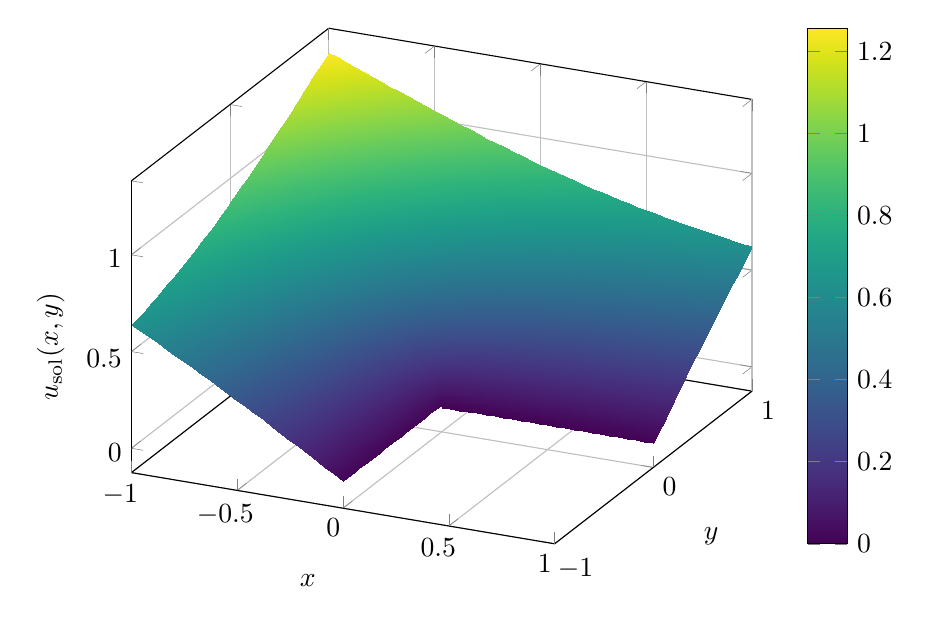
\begin{tikzpicture}
\begin{axis}[
  scale=1.15,
  surf,
  shader=interp,
  grid=major,
  colorbar,
  colormap/viridis,
  xlabel=$x$,
  ylabel=$y$,
  zlabel={$u_\mathrm{sol}(x,y)$}
  ]
% quadrant I
\addplot3[surf,domain=0:1, y domain=0:1] {pow(x*x+y*y,0.33)*sin(0.66*atan(y/x)))};

% quadrant II
\addplot3[surf,domain=-1:0, y domain=0:1] {pow(x*x+y*y,0.33)*sin(0.66*(atan(y/x)+180))};

% quadrant III
% add offset to close interpolation gap
\addplot3[surf,domain=-1:0, y domain=-1:0] {pow(x*x+y*y,0.33)*sin(0.66*atan(x/y)) + 0.014};
\end{axis}
\end{tikzpicture}